\section{Survey}
\label{as:survey}

In this section, we provide further information about the survey presented in Sec.~\ref{sec:survey} that guided our benchmark development. We'll discuss how we selected activities that are part of the survey, the survey design and execution, and the demographic information about the survey participants.

\subsection{Activity Sources} 
We source activities from a combination of \textit{time-use surveys} and WikiHow~\cite{koupaee2018wikihow}. Time-use surveys are studies that inquire about the daily time use of a population~\cite{atus}, making them a good proxy for daily requirements of embodied intelligence. We combine information from three time-use surveys\textemdash American~\cite{atus}, Harmonized European~\cite{hetus}, and Multinational~\cite{mtus} Time Use Surveys\textemdash and obtain an initial set of 540 activities. 
The time-use surveys focus on activities that happen with enough frequency and require a significant amount of time. However, there are other activities that are essential for everyday human life, but not reflected in the time-use surveys.
WikiHow articles include activities that are important for humans where they seek guidance, even if they are not as frequent as the ones included in the time-use surveys. 
This indicates a great potential to source additional useful and relevant daily activities. 
We complement the activities from the time use surveys with WikiHow article titles, of which there are 180,000+. These constitute a raw set of activities that are filtered down by feasibility, as explained in the next paragraph. 

\paragraph{Activity filtering for feasibility:} Simulation constrains which activities collected from time-use surveys and WikiHow can actually be used in \benchmark. We used the following criteria based on \simulator and \bddl constraints to filter the activity pool prior to the survey: 

\begin{table}[h]
    \centering
    \label{tab:xxxx}
    \resizebox{\textwidth}{!}{%
\begin{tabular}{|l|l|}
    \hline
    \textbf{Filtering principle} & 
    % \textbf{Reason} & 
    \textbf{Example activity filtered out} \\
    \hline
    Activity requires physics or chemistry not supported in simulation & 
        % Unsimulatable by definition & 
        \texttt{SteamingClothes}, \texttt{MakingSoap} \\
    Activity involves creating or consuming media & 
        %Decision not to simulate media, difficult to represent media content compactly in \bddl &
        \texttt{ReadingABook} \\
    Activity requires more than a day in real time & 
        % Time horizon has potential to be excessive for modern algorithms, and activity is likely to be mostly passive &
        \texttt{DryingSeedsOvernight} \\
    Activity requires non-visual perceptual modalities & 
        % Most simulators, including \simulator, only provide visual signals & 
        \texttt{SweeteningFood} \\
    Activity requires geometric configurations too fine-grained for \bddl &
        % \bddl has only the positional predicates listed in~\ref{tab:supp_preds_table}, making it powerful for expressing general positions but not specific ones & 
        \texttt{SettingUpANativityScene} \\
    Activity is predicated on branded items & 
        % Branding is generally inappropriate for an open-source tool \todo{what's the exact reason here?} & 
        \texttt{SprayingWindex} \\
    Activity involves other people or live animals & 
        % \simulator does not currently support multi-agent use, and current behavior models of both humans and non-human animals are unlikely to be realistic enough to use as ground truth in a benchmark over a long time-horizon and in high-level cognitive activities \\
        \texttt{AskingForARaise}\\
    \hline
\end{tabular}
}
\end{table}
After filtering and eliminating duplicates, and including the activities from~\cite{srivastava2021behavior}, 2,090 activities remain to be surveyed.

% \labelitemii{{\tiny$\bullet$}}
\subsection{Survey Design} 
Our survey is structured as follows:
\vspace{-2mm}
\begin{itemize}[leftmargin=1.5em]
    % \item Survey respondent reads instructions, which say ``What activities would you like done by a robot? Let's assume that this robot can do any activity well. For each activity, tell us how much you would like a robot to complete it for you.'', followed by detailed instructions describing the question format and illustrative examples.
    \item \textbf{Demographic questions} requesting information about the number of people in the household, occupation, general location, and relationship between household work, automation, and livelihood (see Fig.~\ref{fig:activity_survey_demo} for results). 
    \item \textbf{Activity survey questions} requesting the value of automation of a batch of activities to the respondent. Specifically, this section comprises:
    \begin{itemize}
        \item 50 questions, one question per activity 
        \item Question text: \textit{On a scale of 1 (left) to 10 (right), rate how much you want a robot to do this activity for you.}
        \item Each response uses an independent Likert score~\cite{likert1932technique} on a scale from 1 (less beneficial) to 10 (most beneficial)
    \end{itemize}
\end{itemize}

We piloted alternatives for the survey about two design decisions: 1) question wording, and 2) question format. With respect to the wording for the question, we piloted three alternatives to specify the \textit{agent}: \textit{robot}, \textit{assistant}, and \textit{automation}. Our goal was to study any possible (mis)conceptions about robots that might bias the study. By way of 30 pairwise T-tests and 10 ANOVAS~\cite{stats2013montgomery}, we did not find any statistically significant difference between the results obtained using these three wordings. With respect to the format of the question, we piloted two alternative formats: 10-point Likert, and three-element best-worst scaling. By way of Kendall's tau~\cite{stats2013montgomery}, there was a strong correlation between the rankings determined by Likert scores and standard metrics of best-worst scaling. We, therefore, conclude that either method will give us a similar ranking, and select the more resource-efficient option (Likert). 

\paragraph{Survey collection:}
We deployed our survey on Amazon Mechanical Turk~\cite{paolacci2010running} and collected 50 unique responses per activity. There were a total of 1,461 different respondents and their average scores ranged from 1.9 to 9.3, showing high diversity. The average score was 5.16. To ensure response quality, we repeated four questions in every survey as an attention check. If responses to a pair of repeats differed by more than two points, we considered it failed. Two or more failures led to rejection. We also rejected survey responses that had no significant variance across their responses to 50 different activities.

% ROBERTO: Commenting out this plot. It is unclear the information that it provides. If we want to include it back, we should fix the ticks in the x axis and include more activities, right now it takes too much space to just show 20 numbers (scores)
% \begin{figure}[t]
%     \centering
%     \includegraphics[width=\textwidth]{figures/survey/evenspace20.pdf}
%     \caption{Results of the activity preference survey for twenty activities. The activities are evenly spaced throughout the entire ranking of 1,990 activities.}
%     \label{fig:activity_survey_responses}
% \end{figure} 

\subsection{Demographic Information}
\label{sec:demographics}

Fig.~\ref{fig:activity_survey_demo} depicts the results of our demographic questions on the participants of the survey. We observe that most adult age groups have good representation, particularly pre-retirement age groups, and are concentrated in the 30-40 group. Racially, the respondents are around 75\% white, a larger proportion than the U.S. population but similar to the Mechanical Turk proportion~\cite{pew2016mturkdemog}. Other races appear to have proportions similar to but not the same as their presence on both Mechanical Turk and in the general population; this may be due to their overall small numbers in all three~\cite{pew2016mturkdemog}. There is some Native American representation, though not statistically significant. Income-wise, respondents tend to be in the \$30,000-\$150,000 range, particularly in the lower half. 

The participants' gender is distributed by 43.41\% women, 55.50\% men, 0.83\% non-binary, 0.26\% other. Gender representation is not as even as the U.S. population but more so than the Mechanical Turk worker population~\cite{pew2016mturkdemog}. There is a small representation of non-binary individuals. When it comes to disability status, our participants reported 92.56\% no-disability, 5.74\% disability, and 1.70\%
prefer not to answer. Thus, our survey contained some but limited representation of people with disabilities. This group, together with the elderly, are groups commonly assumed to potentially benefit from robotic efforts; they could be subject to future targeted surveys.

\begin{figure}[t!]
\centering
% \begin{subfigure}[t]{0.3\textwidth}
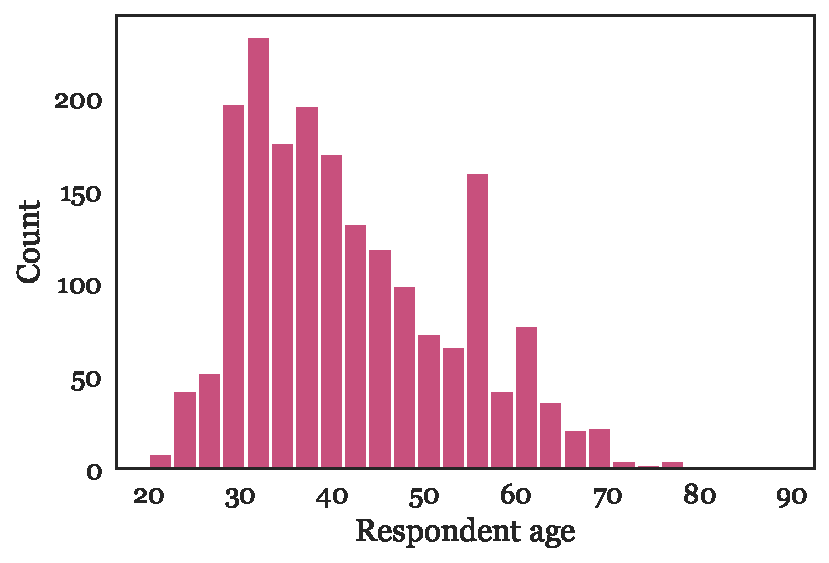
\includegraphics[width=0.33\textwidth,valign=T]{figures/survey/age.pdf}%
% \caption{Age}
% \end{subfigure}
\hfill%
% \begin{subfigure}[t]{0.3\textwidth}
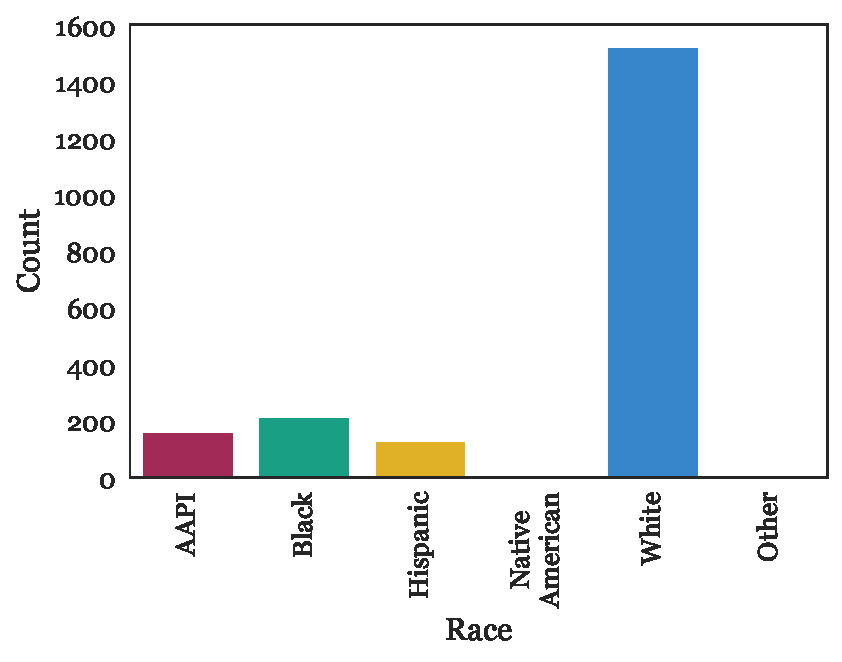
\includegraphics[width=0.33\textwidth,valign=T]{figures/survey/race.pdf}%
% \caption{Race}
% \end{subfigure}
\hfill%
% \begin{subfigure}[t]{0.30.33\textwidth}
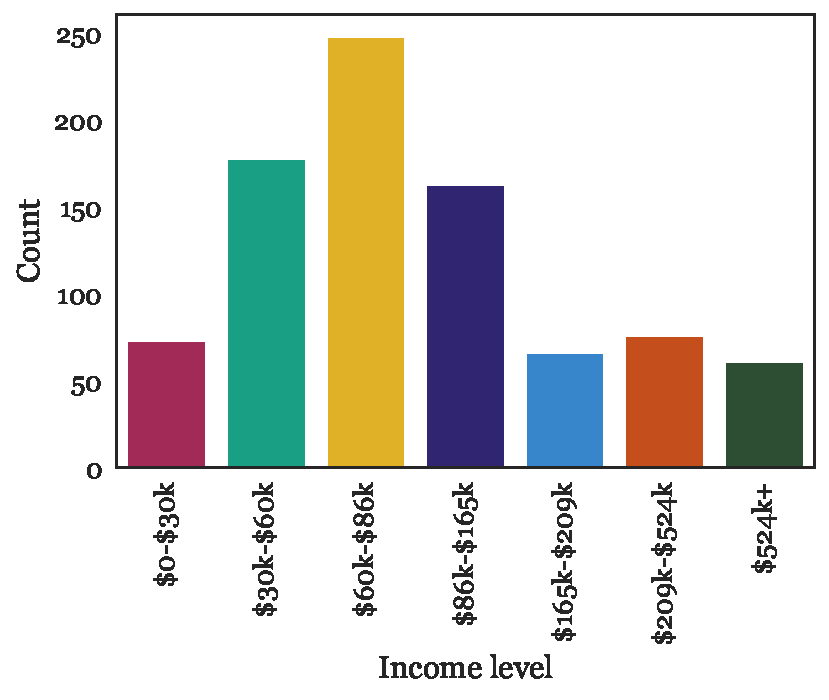
\includegraphics[width=0.33\textwidth,valign=T]{figures/survey/income.pdf}%
% \caption{Income}
% \end{subfigure}
% \\
% \begin{subfigure}[t]{0.3\textwidth}
%     \includegraphics[width=\textwidth]{figures/survey/gender.pdf}
% \caption{Gender}
% \end{subfigure}
% % \hfill
% \begin{subfigure}[t]{0.3\textwidth}
%     \includegraphics[width=\textwidth]{figures/survey/disability.pdf}
% \caption{Disability status}
% \end{subfigure}
\caption{\textbf{Demographic distribution of the participants in our survey.} Respondents appear to have similar demographics to the wider U.S. Mechanical Turk worker population~\cite{pew2016mturkdemog}. Not pictured: respondent gender (43.41\% women, 55.50\% men, 0.83\% non-binary, 0.26\% other), disability status (92.56\% no, 5.74\% yes, 1.70\% prefer not to answer).}
\label{fig:activity_survey_demo}
\end{figure}

\section{Activity Annotation}
\label{as:act_ann}
Obtaining the \bddl definitions for 1,000 activities requires multiple preparatory steps to gather the knowledge needed. This knowledge also becomes part of the~\dataset. The pipeline is outlined in Fig.~\ref{fig:activity_pipeline}. We now detail each annotation other than the survey. Furthermore, quality assessment statistics for these annotations are found in Sec.~\ref{sec:annot_qa}. We see that experienced annotators find our resulting \benchmark knowledge base highly accurate.

\begin{figure}[t]
    \centering
    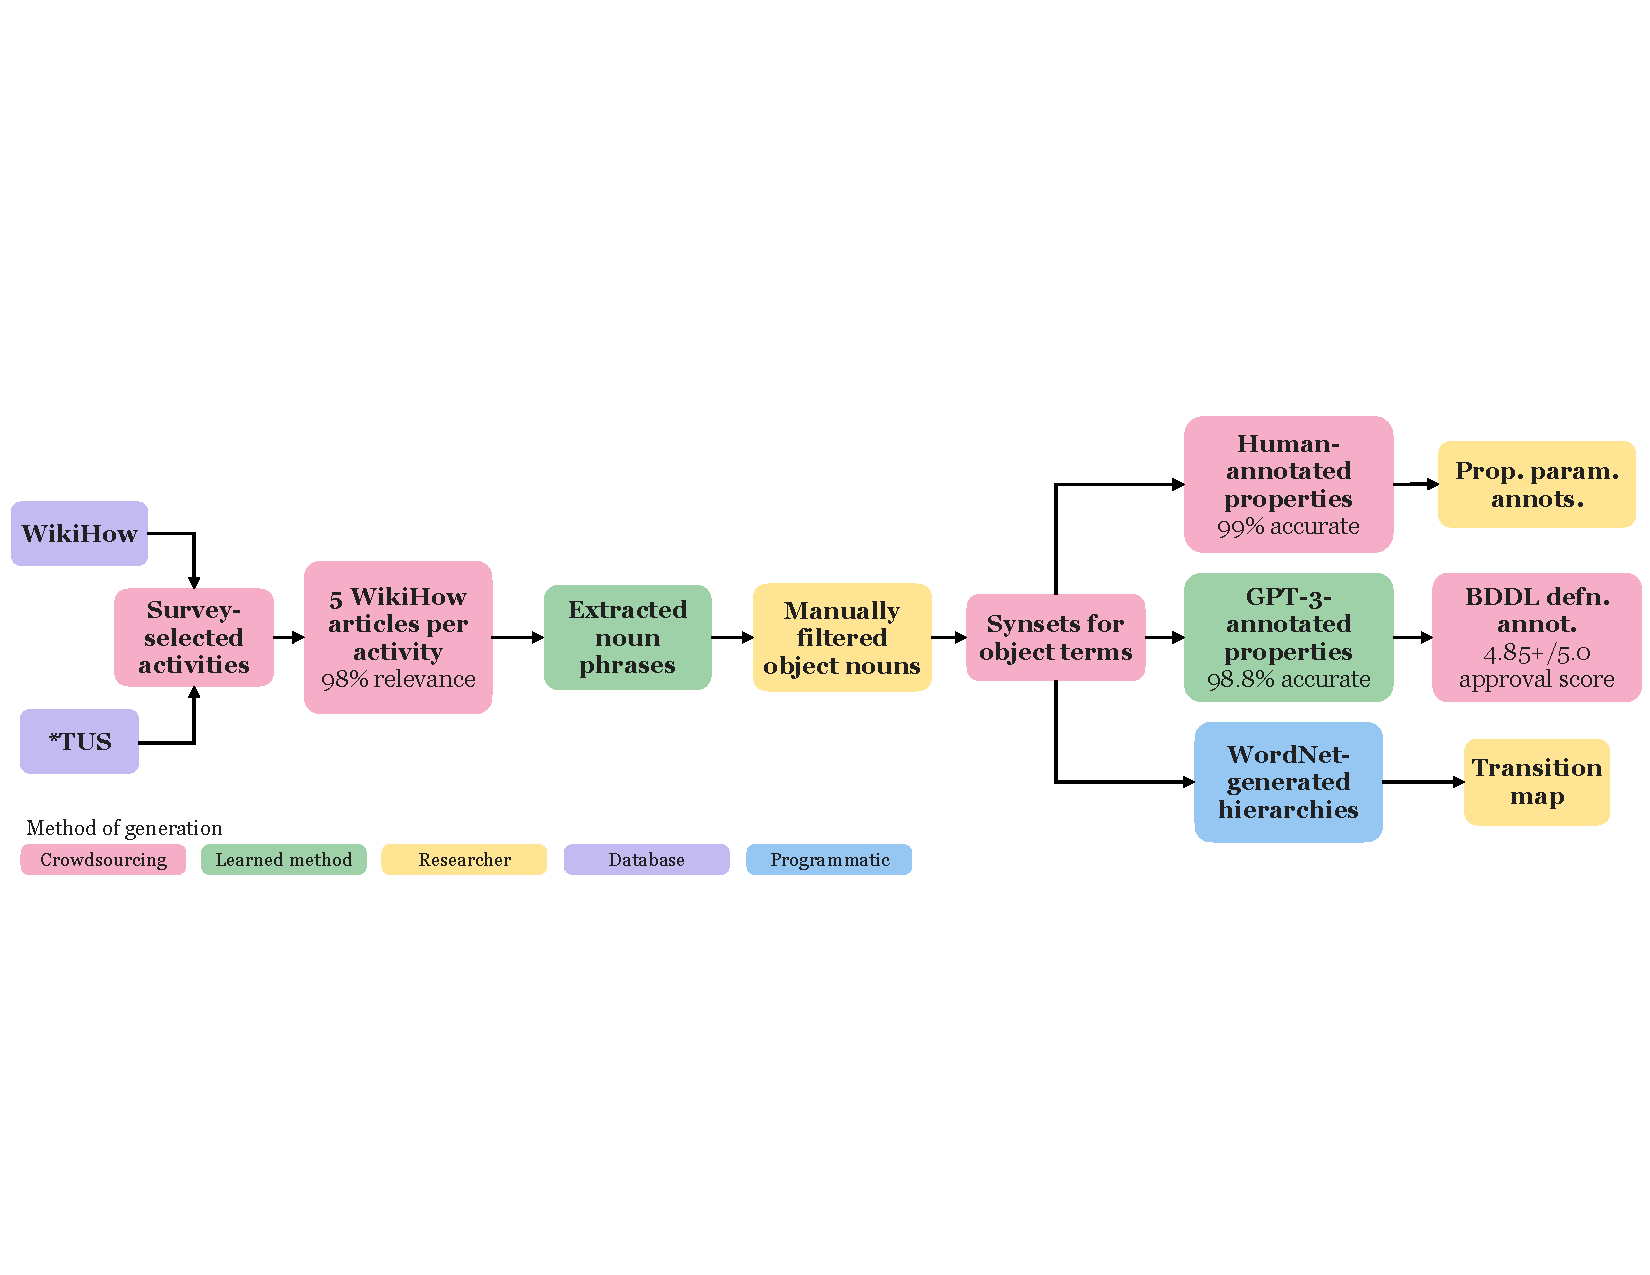
\includegraphics[width=\textwidth]{figures/activities/pipeline.pdf}
    \caption{\textbf{Flow chart of the annotation pipeline:} activity selection, activity article collection, object list extraction, object property and parameter annotation, \bddl annotation.}
    \label{fig:activity_pipeline}
\end{figure}

\paragraph{Obtaining list of objects per activity (WikiHow articles, noun phrase extraction, and manual object filtering):} Our activity definition requires first defining a set of objects and properties that the annotators could use to describe an activity. We would like these domains to be natural and ecological, containing all relevant objects that humans may consider necessary for a task. To obtain such an ecologically plausible object space per activity, we parse WikiHow articles. Since WikiHow is a how-to database with a wide following and community as well as expert- and peer-review, the article texts document objects that are used and acted on in an activity. We therefore asked crowdworkers from the Upwork platform to collect articles; for robustness, we had five articles collected for each activity. We used a chunking model~\cite{akbik2018coling} to extract noun phrases from the article text, then we manually filtered the noun phrases into tangible objects. 

\paragraph{Synsets for object terms and WordNet hierarchy generation:} After obtaining an object space for each activity, we take their union and crowdworkers match each one to a WordNet~\cite{wordnet} synset. This eliminates word-sense ambiguity in the knowledge base and creates a hierarchical structure in the overall object space via the WordNet hierarchy. This process yielded 1,538 total WordNet leaf synsets. Based on various property annotations and needs of the activity set, there are also 1,426 custom synsets for a total of 2,964 leaf synsets.

\paragraph{Property annotations:} Each object that is a leaf-level synset of the WordNet hierarchy is associated with the set of object properties in \benchmark, each of which is fully simulatable in \simulator (full list of properties in Table~\ref{tab:supp_props}). The properties define which predicates can apply to the object - e.g. an object having the \texttt{cookable} property means it can be \texttt{cooked} and \texttt{not cooked}. This association is done task-agnostically because objects/states that are irrelevant or undesirable for a specific activity will still provide important learning signals. All properties that apply to many of the 2,964 leaf synsets and therefore require a large-scale annotation are done by either GPT-3~\cite{gpt3} or crowdworkers. GPT-3 is used for all properties (total of eight) for which the Hamming distance and false-positive rate for a sample compared to a human-annotated ground-truth are both less than 10\%. Human annotation is used for five more properties. The remaining properties are either sensitive to the simulator implementation and are therefore annotated manually, or can be inferred from the other annotations and are determined analytically. 

This annotation is done only for leaf-level synsets, then properties of higher-level synsets are inferred from the leaf-level annotations. This prevents definition unsolveability. In more detail: as shown in Fig.~\ref{fig:activity_pipeline}, the hierarchical structure is applied to the object space. This allows activity definition annotators to refer to them instead of leaf-level synsets; for example, a \texttt{PuttingAwayGroceries} definition can have ``five \texttt{edible\_fruit.n.01}s'' rather than ``two \texttt{apple.n.01}s and three \texttt{banana.n.01}s'', allowing more variation in activity instantiation because far more object models are valid. However, 3-D object models are generally only attached to leaf- or near-leaf-level synsets, meaning that a definition may have a higher-level synset with various predicates attached to it, and at simulation time the object model (associated with one of the synset's descendants) must have those states simulated. A problem might occur when e.g. \texttt{container.n.01} is annotated as \texttt{fillable} and the definition calls for a \texttt{container.n.01} to be \texttt{filled} with a \texttt{liquid}, but the actual model that gets sampled into the simulator to satisfy \texttt{container.n.01} is a cloth bag that doesn't support being \texttt{filled} with a \texttt{liquid}. So to avoid this unsolveability, the properties of any non-leaf synset are exactly the \textit{intersection of all its descendants' properties}.

%\begin{table}[t]
% \centering
% \resizebox{\textwidth}{!}{%
{\scriptsize
\centering
\begin{longtable}{|l|p{.20\textwidth}|p{.25\textwidth}|p{.28\textwidth}|}
        \hline
        \textbf{Object property} & \textbf{Annotation method} & \textbf{Prompt to annotator} & \textbf{Example objects}
        \\\hline
        \texttt{assembleable} & 
            manual &
            N/A & 
             \texttt{desk.n.01},  \texttt{table.n.02}
        \\\hline
        % \texttt{boilable} & 
        %     prog. (all \texttt{liquid}) &
        %     N/A & 
        %      \texttt{champagne.n.01},  \texttt{beef\_broth.n.01}
        % \\\hline
        \texttt{breakable} & 
            human &
            %  Mark if the object can \\be broken into smaller pieces \\by a human dropping it \\on the floor without a tool.\end{tabular} &
            Mark if the object can be broken into smaller pieces by a human dropping it on the floor without a tool.  & 
              \texttt{wine\_bottle.n.01}, \texttt{room\_light.n.01} 
        \\\hline
        % \texttt{cleaningTool} & 
        %     GPT-3 &
        %     %  Is a [object] designed \\to clean things?\end{tabular} & 
        %     Is a [object] designed to clean things? &
        %      \texttt{scrub\_brush.n.01}, \texttt{pipe\_cleaner.n.01}
        % \\\hline
        \texttt{cloth} & 
            manual &
            N/A & 
             \texttt{hammock.n.02}, \texttt{canvas.n.01} 
        \\\hline
        \texttt{coldSource} & 
            GPT-3 &
            Is [object] a source of cold? & 
             \texttt{refrigerator.n.01}, \texttt{ice.n.01}
        \\\hline
        \texttt{cookable} & 
            GPT-3 &
            Can a [object] be cooked? & 
             \texttt{biscuit.n.01},
            \texttt{pizza.n.01}
        \\\hline
        \texttt{deformable} & 
             prog. (all \texttt{softBody}, \texttt{cloth}, \texttt{rope}) &
            N/A & 
              \texttt{tortilla.n.01},  \texttt{clay.n.01} 
        \\\hline
        \texttt{diceable} & 
             prog. (all \texttt{sliceable}'s derivative synsets &
            N/A & 
              \texttt{half\_\_apricot.n.01},  \texttt{half\_\_brisket.n.01} 
        \\\hline
        \texttt{drapeable} & 
             prog. (all \texttt{cloth}, \texttt{rope} &
            N/A & 
              \texttt{dress.n.01},  \texttt{bath\_towel.n.01} 
        \\\hline
        \texttt{fillable} & 
             manual &
            N/A & 
              \texttt{stockpot.n.01},  \texttt{bucket.n.01} 
        \\\hline
        \texttt{fireSource} & 
            GPT-3 &
            %  Is a [object] designed \\to create fire?\end{tabular} & 
            Is a [object] designed to create fire? & 
             \texttt{lighter.n.01}, \texttt{sparkler.n.01} 
        \\\hline
        \texttt{flammable} & 
            human &
            %  Mark if the object can \\catch fire (i.e. burn with \\a flame). For example, \\'wood' and 'gasoline' are \\\textbf{flammable}.\end{tabular}  & 
            Mark if the object can catch fire (i.e. burn with a flame). &
             \texttt{candle.n.01}, \texttt{mail.n.01}
        \\\hline
        \texttt{foldable} & 
             prog. (all \texttt{cloth}, \texttt{softBody}) &
            N/A & 
             \texttt{tortilla.n.01}, \texttt{jean\_jacket.n.01} 
        \\\hline
        \texttt{freezable} & 
             prog. (all \texttt{heatable}) &
            N/A & 
             \texttt{olive\_oil.n.01}, \mbox{\texttt{ginger\_beer.n.01}}
        \\\hline
        \texttt{heatable} & 
            prog. (all rigid bodies) &
            N/A & 
             \texttt{oil.n.01}, \texttt{fish\_knife.n.01} 
        \\\hline
        \texttt{heatSource} & 
            GPT-3 &
            Is a [object] a source of heat? & 
             \texttt{oven.n.01}, \texttt{toaster.n.01} 
        \\\hline
        \texttt{liquid} & 
            GPT-3 &
            Is a [object] a liquid? & 
             \texttt{gasoline.n.01}, \mbox{\texttt{liquid\_soap.n.01}} 
        \\\hline
        \texttt{macroPhysicalSubstance} & 
            manual &
            N/A & 
             \texttt{grated\_cheese.n.01}, \texttt{blueberry.n.02} 
        \\\hline
        \texttt{meltable} & 
            manual &
            N/A & 
             \texttt{cheese.n.01}, \texttt{chocolate.n.02} 
        \\\hline
        \texttt{microPhysicalSubstance} & 
            manual &
            N/A & 
             \texttt{brown\_sugar.n.01}, \texttt{cinnamon.n.03} 
        \\\hline
        \texttt{mixingTool} & 
            manual &
            N/A & 
             \texttt{putty\_knife.n.01}, \texttt{teaspoon.n.02} 
        \\\hline
        \texttt{needsOrientation} & 
            manual &
            N/A & 
             \texttt{cumin\_\_shaker.n.01}, \texttt{salt\_\_shaker.n.01} 
        \\\hline
        \texttt{openable} & 
            human &
            %  Mark if the object is \\designed to be opened.\end{tabular}  & 
            Mark if the object is designed to be opened. &
             \texttt{mixer.n.04}, \texttt{keg.n.01} 
        \\\hline
        \texttt{particleApplier} & 
            manual &
            %  Mark if the object is \\designed to be opened.\end{tabular}  & 
            N/A &
             \texttt{pepper\_mill.n.01}, \texttt{detergent\_\_atomizer.n.01} 
        \\\hline
        \texttt{particleRemover} & 
            GPT-3 &
            %  Mark if the object is \\designed to be opened.\end{tabular}  & 
            Can a [object] absorb liquid? &
             \texttt{scrub\_brush.n.01}, \texttt{broom.n.01} 
        \\\hline
        \texttt{particleSource} & 
            manual (on top of \texttt{particleApplier} &
            %  Mark if the object is \\designed to be opened.\end{tabular}  & 
            N/A &
             \texttt{sink.n.01}
        \\\hline
        \texttt{particleSink} & 
            manual (on top of \texttt{particleRemover} &
            %  Mark if the object is \\designed to be opened.\end{tabular}  & 
            N/A &
             \texttt{sink.n.01}
        \\\hline
        % \texttt{overcookable} & 
        %      prog. (all \texttt{cookable}) &
        %     N/A & 
        %      \texttt{gazpacho.n.01}, \texttt{jam.n.01}
        % \\\hline
        % \texttt{physicalSubstance} & 
        %     manual &
        %     N/A & 
        %      \texttt{flour.n.01}, \texttt{salt.n.02} 
        % \\\hline
        \texttt{rigidBody} & 
            manual &
            N/A & 
             \texttt{tomato.n.01}, \texttt{desk.n.01} 
        \\\hline
        \texttt{rope} & 
            manual &
            N/A & 
             \texttt{ribbon.n.01}, \texttt{fairy\_light.n.01} 
        \\\hline
        \texttt{sliceable} & 
            GPT-3 &
            %  Can a [object] be sliced \\easily by a human \\with a knife?\end{tabular} & 
            Can a [object] be sliced easily by a human with a knife? &
             \texttt{sweet\_corn.n.01}, \mbox{\texttt{sandwich.n.01}} 
        \\\hline
        \texttt{slicingTool} & 
            GPT-3 &
            Can a [object] slice an apple? & 
             \texttt{blade.n.09}, \texttt{razor.n.01}
        \\\hline
        % \texttt{soakable} & 
        %     GPT-3 &
        %     Can a [object] absorb liquid? & 
        %      \texttt{sponge.n.01}, \texttt{tea\_bag.n.01}
        % \\\hline
        \texttt{softBody} & 
            manual &
            N/A & 
             \texttt{dough.n.01}, \texttt{pillow.n.01} 
        \\\hline
        \texttt{substance} & 
             prog. (all \texttt{liquid}, \texttt{vis.Subst.}, \texttt{phys.Subst.}) &
            N/A & 
             \texttt{water.n.06}, \texttt{milk.n.01} 
        \\\hline
        \texttt{toggleable} & 
            human &
            %  The object can be switched \\between a finite number \\of \textit{discrete} states and is \\designed to do so.\end{tabular} & 
            The object can be switched between a finite number of \textit{discrete} states and is designed to do so. &
            %  \texttt{hot\_tub.n.01}, \\ \texttt{light\_bulb.n.01}\end{tabular} \\
            \texttt{hot\_tub.n.01}, \texttt{light\_bulb.n.01} 
        \\\hline
        \texttt{unfoldable} & 
            prog. (all \texttt{foldable}) &
            N/A & 
             \texttt{tissue.n.02}, \texttt{foil.n.01} 
        \\\hline
        \texttt{visualSubstance} & 
            manual &
            N/A & 
             \texttt{coriander.n.02}, \mbox{\texttt{cocoa\_powder.n.01}}
        \\\hline
        \texttt{waterCook} & 
            manual (special case of \texttt{cookable} &
            N/A & 
             \texttt{chickpea.n.01}, \mbox{\texttt{white\_rice.n.01}}
        \\\hline
        % \texttt{waterSource} & 
        %     manual &
        %     N/A & 
        %     \texttt{sink.n.01} 
        % \\\hline
        % \texttt{wetable} & 
        %     prog. (all non-\texttt{substance} &
        %     N/A & 
        %      \texttt{lasagna.n.01}, \texttt{ashtray.n.01}
        % \\\hline
    % \end{tabular}
    \caption{Properties annotated for \benchmark for each object category and included in the \dataset knowledge base}
    \label{tab:supp_props}
\end{longtable}
}
%\end{table}


\paragraph{Property parameter annotations:} \bddl separates objects and object states (i.e. terms and predicates), but simulating realistic ``cooking'' or ``filling'' requires information for object-object property tuples, not just objects or object properties alone. For example, in the real world, an \texttt{apple.n.01} and a \texttt{chicken.n.01} do not become cooked at the same temperature, so simply knowing they are both \texttt{cookable} is insufficient. \dataset therefore includes manual annotation of several property parameters that are (object, object property) specific, such as \texttt{cookTemperature} for all \texttt{cookable} objects. 

Examples of object-property pairs and parameters:
\vspace{-2mm}
\begin{itemize}[leftmargin=2em]
    \item Temperature required for \texttt{cookable} object to go from \texttt{(cooked object) = False} to \texttt{(cooked object) = True}
    \begin{itemize}
        \item \texttt{crab.n.05}: must reach \textbf{63\textdegree C}
        \item \texttt{squash.n.02}: must reach \textbf{58\textdegree C}
         \item \texttt{meatball.n.01}: must reach \textbf{63\textdegree C}
        \item \texttt{chicken\_leg.n.01}: must reach \textbf{74\textdegree C}
    \end{itemize}
    \item Temperature generated by \texttt{heatSource} object. For \texttt{toggleable heatSource}s, this may require \texttt{toggledOn(object) = True}
    \begin{itemize}
        \item \texttt{toaster\_oven.n.01}: generates \textbf{204\textdegree C}
        \item \texttt{ember.n.01}: generates \textbf{1093\textdegree C}
        \item \texttt{hand\_blower.n.01}: generates \textbf{45\textdegree C}
        \item \texttt{coffee\_maker.n.01}: generates \textbf{93\textdegree C}
    \end{itemize}
\end{itemize}



\paragraph{Transition rules:} There are many activities that involve complex chemical and physical processes that are beyond the capability of the state-of-the-art simulation technology. For example, blending different fruits into a smoothie or sanding a rusted surface are extremely difficult to simulate, but the agent actions to complete these tasks are still within reach, e.g. placing the fruits inside a blender. Therefore, in ordet to support these type of activities, we create a set of transition rules that will be used by \simulator to bypass the underlying physics but still produce visually realistic physical transitions, e.g. smoothie particles being generated inside the blender after the blender is turned on.

%simulation, but executing them realistically does not require a deep understanding of those. For example, only certain cleansing agents can clean up grease while many more can clean up the dust. Enforcing this constraint through pure simulation is beyond most state-of-the-art simulators, but for any agent (including a human) that has been given the right materials, the processes are very similar. So, we create a set of transition rules activities including cooking, cleaning, and assembly to make such activities possible and ensure that they require realistic agent actions.

Examples of transition rules: 
\vspace{-2mm}
\begin{itemize}[leftmargin=2em]
    \item Composition and decomposition of objects 
    \begin{itemize}
        \item Transition rule used in \texttt{make a strawberry slushie}
        \begin{itemize}
            \item \textbf{Inputs:} \texttt{strawberry.n.01}, \texttt{ice.n.01}, \texttt{lemon\_juice.n.01}, \texttt{agave.n.01}
            \item \textbf{Transition machine:} \texttt{blender.n.01}
            \item \textbf{Outputs:} \texttt{smoothie.n.01}
        \end{itemize}
        \item Transition rule used in \texttt{make gazpacho}
        \begin{itemize}
            \item \textbf{Inputs:} \texttt{basil.n.03}, \texttt{salt.n.02}, \texttt{black\_pepper.n.02}, \texttt{tomato\_juice.n.01}, \texttt{cucumber.n.02}, \texttt{water.n.06}, \texttt{lemon\_juice.n.01}
            \item \textbf{Transition machine:} \texttt{saucepan.n.01}
            \item \textbf{Outputs:} \texttt{gazpacho.n.01}
        \end{itemize}
    \end{itemize}
    \item Realistic cleaning rules
    \begin{itemize}
    \item Transition rule used in \texttt{CleanTheExteriorOfYourGarage}
    \begin{itemize}
        \item \textbf{Substance covering object:} \texttt{paint.n.01} or \texttt{spray\_paint.n.01}
        \item \textbf{Objects needed to remove:} \texttt{particleRemover} saturated with (\texttt{solvent.n.01} or \texttt{acetone.n.01})
    \end{itemize}
    \item Transition rule used in \texttt{CleanYourRustyGardenTools}
    \begin{itemize}
        \item \textbf{Substance covering object:} \texttt{rust.n.01} or \texttt{patina.n.01} or \texttt{incision.n.01} (simulated as particles but exposed to annotators as unary \texttt{scratched} predicate) or \texttt{tarnish.n.01} (simulated as particles but exposed to annotators as unary \texttt{tarnished} predicate)
        \item \textbf{Objects needed to remove:} \texttt{emery\_paper.n.01} or \texttt{whetstone.n.01}
    \end{itemize}
    \end{itemize}
\end{itemize}

\paragraph{Activity definitions in \bddl:} Finally, the object spaces and the relevant properties and predicates they enable are offered to lay annotators to generate \bddl definitions. Annotators build activity definitions using an annotation interface that includes a visual version of \bddl~\cite{srivastava2021behavior} (details on new features in \bddl are in  Sec.~\ref{sec:bddl}). The annotation interface enforces the requirements needed to make definitions logically solvable and well-formed. We collect one definition per activity for a total of 1,000 \bddl activity definitions.

Listings~\ref{lst:bddl3},~\ref{lst:bddl4}, and~\ref{lst:bddl5} show examples of \benchmark activity definitions, while Listing~\ref{lst:bddl1} and~\ref{lst:bddl2} show examples of \oldbenchmark definitions. We see that while the numbers of objects and literals are similar, speaking to the fact that both benchmarks have reached similar scale and detail for the activities they have, \benchmark has far larger and more detailed activity distribution. The \texttt{BakingSugarCookies} activity involves transition rules that turn ingredients in \texttt{:init} to scones in \texttt{:goal}, a process that will require the listed mixer and oven in \simulator. By contrast, cooking in \oldbenchmark was limited to single objects transitioning from \texttt{not cooked} to \texttt{cooked}; other benchmarks are similar or lack cooking entirely. \texttt{CleanYourLaundryRoom} involves specific cleansing agents to clean mold, whereas \oldbenchmark cleaning tasks only had two types of ``dirtiness'' (\texttt{stained} and \texttt{dusty}) and the only rule was to use water in the case of \texttt{stained}. \texttt{CleanTheBottomOfAnIron} also shows rust-specific cleaning (requiring emery paper).

\subsection{Quality assessment of \benchmark annotations}
\label{sec:annot_qa}
% TODO 

\begin{table}[h]
    \centering
     \resizebox{\textwidth}{!}{  
    \begin{tabular}{|c|c|c|c|c|}
        \hline
        & Article Collection & Object Extraction & Human Properties & GPT-3 / Machine Properties \\ %& Parameter Annotation &  Activity Definition \\
         \hline
        Accuracy (Approval Rate)  & 0.974 & 0.968 & 0.990 & 0.988 \\ % & & \\
        \hline
        F1-score & 0.984 & 0.990 & 0.912 & 0.930 \\ % & & \\
        \hline
        False Discovery Rate & 0.026 & 0.032 & 0.031 & 0.029 \\ % & & \\
        \hline
        False Positive Rate & N/A & N/A & 0.002 & 0.003 \\ % & & \\
        \hline
    \end{tabular}}
    \caption{Quality check results for object and object property annotations: for each stage in the annotation pipeline, report human verification results. The F1-score is $\frac{2}{\texttt{precision}^{-1} + \texttt{recall}^{-1}}$. The False Discovery Rate is FDR = FP/(TP+FP) and the False Positive Rate FPR = FP/(TN+FP). The high accuracy and F1-scores and low FDRs and FPRs show that our annotation results are of high quality. }
    \label{tab:activity_qc}
\end{table}

\begin{table}[h]
    \centering
     \resizebox{10cm}{!}{  
    \begin{tabular}{|c|c|c|c|c|}
    \hline
    %    \hline
    & \multicolumn{4}{c|}{Activity Definition} \\
        %\cline{1-8}
        \hline
        & Question 1 & Question 2 & Question 3 & Question 4\\ %& Parameter Annotation &  Activity Definition \\
         \hline
        Average Rating  & 4.875 & 4.942 & 4.967 & 4.975 \\ % & & \\
        \hline
        Standard Deviation & 0.331 & 0.234 & 0.364 & 0.156 \\ % & & \\
    \hline
    \end{tabular}}
    \caption{Quality check results for activity definitions. Q1: Are the objects listed relevant to the definition of the task?, Q2: Do the initial placements/locations of objects make sense?, Q3: Are the actions to perform (“goals”) relevant to the definition of the activity?, Q4: Is this definition reasonable?\\ 
    Each activity definition was evaluated on a scale of 1-5 for each of the questions, and the average score and standard deviation are presented. The increased granularity still reflects the high quality of our results.}
    \label{tab:bddl_def_qc}
\end{table}

Our quality control investigation shows us that all labeling done by crowdworkers and GPT-3 is of the highest quality. Five crowdworkers with an extensive background in data labeling for large machine learning projects, coding, or data verification affirmed the results from earlier crowdworkers. The accuracies for all the labeling tasks were all above 96\%, the F1 scores were above 91\% and the false positive and false discovery rates were between 2-3\% as shown in Table~\ref{tab:activity_qc}. We noticed that the Synset Verification is a bit lower in accuracy than the other labeling tasks. This may be due to subtleties in acceptable synset definitions: for example, a ''reasonably narrow hypernym'' of a word not found in WordNet~\cite{wordnet} is acceptable, such as a "dispenser" for a "soap dispenser", but there may be gray areas regarding what is considered "reasonably narrow" (e.g. would a "hand tool" be reasonable as a replacement for a "soap dispenser"?)

The activity definition process was evaluated with more granularity using a Likert scale and an array of questions. We found that the response values had consistently high averages (very close to the maximum score of 5) and low standard deviations as shown in Table~\ref{tab:activity_qc}. We also found no significant discrepancy for activity definition scores across topics (e.g. tasks related to "cleaning"), showing that the \bddl definitions were rated uniformly across the span of activity categories.

\section{New \bddl features}
\label{sec:bddl}

\benchmark uses an expanded version of the~\bddl used in \oldbenchmark~\cite{srivastava2021behavior}, in order to support the new set of diverse activities. There are three new features here: 1) representation of substances, 2) three-valued predicates, and 3) composition and decomposition of objects. %, and 4) variable-arity predicates. We now detail the need for each of these, why the~\bddl from \oldbenchmark cannot support them, and the design in this version of~\bddl.

\paragraph{Representation of substances:} \benchmark introduces \textit{substances}, objects that are arbitrarily subdivideable and do not obey clear instance boundaries such as \texttt{water.n.06} or \texttt{flour.n.01}. The lack of instance boundaries is difficult with traditional PDDL/\bddl: for example, if there are two bottles of orange juice where the juice inside one is called \texttt{orange\_juice.n.01\_1} and the juice inside the other is called \texttt{orange\_juice.n.01\_2}, any mixing of the particles makes it near-impossible for the agent to satisfy a \texttt{:goal} condition pertaining to an instance. Even with quantification, a condition like \texttt{exists (orange\_juice.n.01) (filled orange\_juice.n.01 glass.n.01\_3)} is still unfair: if the agent mixes particles from the two different \texttt{orange\_juice} instances such that together they \texttt{filled glass.n.01\_3} but neither instance alone has enough particles in \texttt{glass.n.01\_3} to fill it, the \texttt{:goal} will not be met.

We simply enforce that there is up to one instance of any \texttt{substance} in a definition. The annotator can still control quantity by spawning it in as many containers as desired. Unlike labeling every particle separately, this maintains a compact representation. This does not allow for some of the substances to be different from some (e.g. some of the orange juice is cold and some is hot), but we consider this an acceptable limitation.

Furthermore, particle-based objects can be computationally expensive to simulate. When an annotator uses \texttt{orange\_juice.n.01} only as a container of orange juice and not actually the particles (e.g. in a \texttt{PuttingAwayGroceries} activity), this becomes a waste of computational resources. Therefore, we introduce a custom container synset for every substance that has the same properties and WordNet hierarchy structure as \texttt{bottle.n.01} and instruct annotators to use it if all they want is the container.

\paragraph{Three-valued predicates:} A common issue in \oldbenchmark activities is that success on predicates involving naturally continuous-valued quantities is sudden and arbitrary: cracking a window a little bit suddenly changes it from \texttt{not open} to \texttt{open}, and the activity from undone to done – even though the window is not a typical human conception of ``open’’. PDDL 2.1~\cite{fox2003pddl21} has numerical fluents and derived predicates, which offer continuous states. However, this granularity may not be crucial to the high-level activities in \benchmark, and the concept is also difficult to communicate to lay annotators.

We therefore treat certain predicates as three-valued by having two Boolean predicates where the negations are the same, such as \texttt{filled} and \texttt{empty} (rather than just \texttt{not filled}). The annotators still see one Boolean predicate, in this case \texttt{filled}, and negate it to say the opposite, but we assume that when they negate, they mean something decisively empty. This is a strong assumption but generally safe as people tend not to add expressions that seem like common sense. Wherever we see the predicate negated in the definition, we switch it out with the other predicate. This applies to \texttt{filled}/\texttt{empty}, \texttt{open}/\texttt{closed}, and \texttt{folded}/\texttt{unfolded}.

To ensure that the definition is logically the same after the switch, the underlying~\bddl implementation converts the definition using De Morgan’s Law such that all negations are only applied to atomic formulae before the switch occurs.

% The only logical pitfall is that the switch does not work for all expressions: \texttt{not (exists (sweater.n.01) (folded sweater.n.01))} is not the same as \texttt{(exists (sweater.n.01) (unfolded sweater.n.01))}
% \texttt{exists (?sweater.n.01) (not (folded sweater.n.01))} is not the same as \texttt{exists (?sweater.n.01) (unfolded sweater.n.01)} – in the first expression, there could be a sweater that is in between \texttt{unfolded} and \texttt{folded}. Instead,  

\paragraph{Composition and decomposition of objects:} In standard PDDL/~\bddl, the objects in \texttt{:objects} are assumed to persist throughout the activity. There is no concept of creating a new object that did not appear in the \texttt{:init} or explicitly destroying an object. 

To enable our transition rules that involve turning some objects into others, we require a representation that will provide the desired information unambiguously. The \texttt{:objects} section cannot be inferred simply from a \texttt{:goal} that has new objects in it, because \texttt{:goal} is not exhaustive. We therefore introduce the \texttt{future} predicate, used in \texttt{:init} on all objects that do not appear in the scene when the agent enters, but must be present for the \texttt{:goal} to be satisfied. All objects in \texttt{future} predicates appear in \texttt{:objects} and they cannot appear in any other literals in \texttt{:init}. This approach takes inspiration from~\cite{wichlacz2019ghost}, which updates a reference to an object (e.g. a wall) as it keeps changing form as more sub-objects (e.g. blocks) are added to it.

% \paragraph{Variable-arity predicates:} Certain predicates can take various numbers of objects while indicating the same underlying concept. For example, in \benchmark, the \texttt{mixed} predicate can take any number of objects: the expressions \texttt{(mixed apple.n.01\_1 apple.n.01\_2 peach.n.03\_1)} and \texttt{(mixed apple.n.01\_1 apple.n.01\_2 peach.n.03\_1 banana.n.01\_1)} give different numbers of objects to \texttt{mixed}, but mean the same thing and are checked the same way in~\simulator. 

% Logic predicates are fixed-arity by default, but work exists to expand to variable-arity predicates~\cite{oliver2004multigrade}. PDDL uses this assumption to specify predicates in its domain that can be used with PDDL actions to create plans. However, because~\bddl is used for benchmarking, it is process-agnostic and does not assume any planning method~\cite{srivastava2021behavior}. Therefore, a domain file does not have any effect in~\bddl, so a variable-arity predicate can be specified (rather than potentially infinite fixed-arity versions) to maintain compactness. This requires no structural changes to~\bddl.



%\begin{longtable}{|p{0.3\textwidth}|p{0.3\textwidth}|p{0.3\textwidth}|}
\hline 1. washing floor & 2. cleaning bathrooms & 3. clean your house after a wild party & 4. cleaning floors \\
\hline 
 5. mopping floors & 6. clean a shower & 7. cleaning toilet & 8. cleaning bathtub \\
\hline 
 9. clean grease & 10. scrubbing bathroom floor & 11. cleaning oven & 12. cleaning stove \\
\hline 
 13. shoveling snow & 14. washing outside windows & 15. clean walls & 16. clean up water damage \\
\hline 
 17. washing dishes & 18. vacuuming floors & 19. picking up trash & 20. clean carpets \\
\hline 
 21. emptying trash cans & 22. cleaning pavement & 23. washing plates & 24. washing outside walls \\
\hline 
 25. cleaning windows & 26. sweeping floors & 27. clean the outside of a house & 28. taking trash outside \\
\hline 
 29. clean a couch & 30. washing pots and pans & 31. remove hard water spots & 32. cleaning barbecue grill \\
\hline 
 33. clean a stainless steel dishwasher & 34. sweeping porch & 35. raking leaves & 36. clean cement \\
\hline 
 37. putting dishes away after cleaning & 38. clean your kitty litter box & 39. washing windows & 40. mopping the kitchen floor \\
\hline 
 41. clean outdoor tiles & 42. remove spots from linen & 43. cleaning microwave oven & 44. clean wood siding \\
\hline 
 45. clean a coffee maker & 46. picking up litter & 47. cleaning up after a meal & 48. clean a drain \\
\hline 
 49. clean a sofa & 50. cleaning vehicles & 51. polish wood floors & 52. clean up after a dinner party \\
\hline 
 53. remove ice from gutters & 54. cleaning carpets & 55. sweeping outside entrance & 56. clean mirrors \\
\hline 
 57. clean a broiler pan & 58. vacuuming vehicles & 59. disposing of lawn clippings & 60. cleaning the pool \\
\hline 
 61. unloading shopping from car & 62. waxing cars or other vehicles & 63. clean a grill pan & 64. mowing the lawn \\
\hline 
 65. cleaning up refrigerator & 66. clean your rusty garden tools & 67. removing ice from walkways & 68. cleaning bedroom \\
\hline 
 69. cleaning debris out of car & 70. sweeping garage & 71. wash towels & 72. washing walls \\
\hline 
 73. washing cars or other vehicles & 74. moving stuff to storage & 75. disposing of trash for adult & 76. assembling furniture \\
\hline 
 77. clearing the table after dinner & 78. clean your laundry room & 79. cleaning up after an event & 80. clean an air filter \\
\hline 
 81. tidying bathroom & 82. cleaning up plates and food & 83. installing carpet & 84. cleaning a car \\
\hline 
 85. cleaning the hot tub & 86. moving boxes to storage & 87. clean up gasoline & 88. clean decking \\
\hline 
 89. clean the exterior of your garage & 90. doing laundry & 91. dusting rugs & 92. clean cups \\
\hline 
 93. clean a mattress & 94. shampooing carpet & 95. clean sheets & 96. cleaning up branches and twigs \\
\hline 
 97. waxing floors & 98. clean kitchen appliances & 99. hoe weeds & 100. storing the groceries \\
\hline 
 101. changing sheets & 102. clean rubber bathmats & 103. clean a chicken coop & 104. scraping snow off vehicle \\
\hline 
 105. cleaning patio furniture & 106. cleaning the yard & 107. folding clean laundry & 108. cleaning driveway \\
\hline 
 109. cleaning kitchen cupboard & 110. folding sheets & 111. clean plastic containers & 112. clean a rug \\
\hline 
 113. clean a vacuum & 114. cleaning cupboards & 115. clean your baseboard radiators & 116. clean stainless steel sinks \\
\hline 
 117. clean a glass windshield & 118. clean household cleaning tools & 119. cleaning garden tools & 120. water your lawn efficiently \\
\hline 
 121. ironing clothes & 122. cleaning fan & 123. chop an onion & 124. clean a toaster oven \\
\hline 
 125. disinfect laundry & 126. cleaning up the kitchen only & 127. chopping wood & 128. painting house exterior \\
\hline 
 129. de-clutter your garage & 130. washing utensils & 131. cleaning garage & 132. laying tile floors \\
\hline 
 133. washing fabrics & 134. washing curtains & 135. folding clothes & 136. unpacking moving van \\
\hline 
 137. clean a kitchen sink & 138. shoveling coal & 139. cleaning freezer & 140. putting away yard equipment \\
\hline 
 141. cleaning pet bed & 142. clean a air conditioner & 143. clean out a guinea pigs hutch & 144. clean up broken glass \\
\hline 
 145. clean a rice cooker & 146. polisha car & 147. clean your cleaning supplies & 148. clean a fish \\
\hline 
 149. bringing laundry & 150. applying pesticides & 151. sweeping patio & 152. cleaning shed \\
\hline 
 153. cleaning closet & 154. cleaning table after clearing & 155. putting away Christmas decorations & 156. cleaning parks \\
\hline 
 157. clean a fence & 158. polishing silver & 159. hanging blinds & 160. doing housework for adult \\
\hline 
 161. cleaning the pond & 162. re-shelving library books & 163. clean couch pillows & 164. putting clean laundry away \\
\hline 
 165. rinsing dishes & 166. sweeping steps & 167. polishing furniture & 168. unloading the car \\
\hline 
 169. putting pesticides on lawn & 170. clean an espresso machine & 171. cleaning around pool in garden & 172. clean the interior of your car \\
\hline 
 173. bringing paper to recycling & 174. clean stucco & 175. spraying for bugs & 176. cleaning lawnmowers \\
\hline 
 177. cleaning tools and equipment & 178. laying wood floors & 179. clean a keyboard & 180. putting laundry in drawer \\
\hline 
 181. treating stains & 182. washing bowls & 183. clean a popcorn machine & 184. clean a dirty tent \\
\hline 
 185. clean a baking stone & 186. organizing boxes in garage & 187. clean up spilled egg & 188. changing dog's water \\
\hline 
 189. cleaning boat & 190. clean reusable shopping bags & 191. clean wood doors & 192. dispose of a pizza box \\
\hline 
 193. drying dishes & 194. clean a faucet & 195. prepare a raised bed garden & 196. loading the dishwasher \\
\hline 
 197. clean brass casings & 198. removing lint from dryer & 199. bringing glass to recycling & 200. making the bed \\
\hline 
 201. clean a patio & 202. laying paving stones & 203. clean the bottom of an iron & 204. putting up wallpaper \\
\hline 
 205. fertilize a lawn & 206. cleaning restaurant table & 207. clean an electric razor & 208. lay sod \\
\hline 
 209. clean a hot water dispenser & 210. clean baking sheets & 211. clean a sauna & 212. clean vinyl shutters \\
\hline 
 213. clean a kitchen table & 214. collecting dishes from restaurant tables & 215. delivering groceries to doorstep & 216. clean flip flops \\
\hline 
 217. taking clothes off of the drying rack & 218. cleaning stuff out of car & 219. installing a fence & 220. store firewood \\
\hline 
 221. wash jeans & 222. clean a light bulb & 223. clean rubber & 224. make coffee \\
\hline 
 225. chopping vegetables & 226. fixing broken table & 227. cleaning camper/RV & 228. organise a linen closet \\
\hline 
 229. wash duvets & 230. stock grocery shelves & 231. clean and disinfect ice trays & 232. clean a hamper \\
\hline 
 233. make cabinet doors & 234. replacing screens & 235. tidying living room & 236. clean a box fan \\
\hline 
 237. clean potatoes & 238. carrying in groceries & 239. cleaning garden path & 240. polish copper \\
\hline 
 241. mulching & 242. hanging up curtains & 243. clean a birdcage & 244. de-ice a car \\
\hline 
 245. polishing shoes & 246. loading shopping into car & 247. clearing table after breakfast & 248. remove scorch marks \\
\hline 
 249. cleaning sneakers & 250. hand washing clothing & 251. clearing table after dinner & 252. washing vegetables \\
\hline 
 253. adding chemicals to lawn & 254. dust houseplants & 255. watering outdoor flowers & 256. turning sprinkler off \\
\hline 
 257. dispose of glass & 258. clean a felt pool table top & 259. putting away toys & 260. painting porch \\
\hline 
 261. spraying fruit trees & 262. putting shopping away & 263. cleaning fishing gear & 264. brushing lint off clothing \\
\hline 
 265. clean a blender & 266. stacking wood & 267. loading the car & 268. sanding wood furniture \\
\hline 
 269. clean a toaster & 270. adding chemicals to pool & 271. remove sod & 272. bringing in wood \\
\hline 
 273. clean a sponge & 274. cleaning shoes & 275. clean a piano & 276. store firewood outdoors \\
\hline 
 277. clean a small pet cage & 278. clean brooms & 279. composting waste & 280. getting package from post office \\
\hline 
 281. picking up toys & 282. fertilizing garden & 283. clean quarters & 284. clean a pickup truck \\
\hline 
 285. picking up baggage & 286. recycling office papers & 287. collecting dishes from around house & 288. clean brass \\
\hline 
 289. disinfect nail clippers & 290. putting away Halloween decorations & 291. clearing table after supper & 292. installing appliances \\
\hline 
 293. sorting bottles, cans, and paper & 294. clean a company office & 295. clean a raincoat & 296. lube a bicycle chain \\
\hline 
 297. dispose of paper & 298. clean place mats & 299. clean leather sandals & 300. unloading shopping items \\
\hline 
 301. putting on license plates & 302. fertilize plants & 303. clean cup holders & 304. wash dog toys \\
\hline 
 305. turning sprinkler on & 306. taking clothes out of the dryer & 307. changing bulbs & 308. tidy your garden \\
\hline 
 309. clean wood pallets & 310. clean your electronics & 311. unpacking car for trip & 312. locking every door \\
\hline 
 313. clearing table after snacks & 314. haul a motorcycle & 315. clean a garden sprayer & 316. clean a whiteboard \\
\hline 
 317. recycling newspapers & 318. fill a punching bag & 319. packing moving van & 320. picking up take-out food \\
\hline 
 321. defrosting freezer & 322. line kitchen shelves & 323. clean black rims & 324. recycling glass bottles \\
\hline 
 325. unloading groceries & 326. putting protective cover on vehicle & 327. putting up shelves & 328. sorting laundry \\
\hline 
 329. clean a backpack & 330. carrying out garden furniture & 331. hanging clothes & 332. cleaning glasses off bar \\
\hline 
 333. clean clear plastic & 334. ironing bedsheets & 335. prepare your garden for winter & 336. chlorinating the pool \\
\hline 
 337. hanging clothes on clothesline & 338. putting clothes into closet & 339. putting up Christmas lights outside & 340. clean soot from glass lanterns \\
\hline 
 341. clean a golf club & 342. watering outdoor plants & 343. putting leftovers away & 344. returning consumer goods \\
\hline 
 345. fixing mailbox & 346. hooking up trailer to car & 347. clean a computer monitor & 348. clean pottery \\
\hline 
 349. putting towels in bathroom & 350. clean a dirty baseball & 351. tidying bedroom & 352. repairs to furniture \\
\hline 
 353. cook chicken and rice & 354. clean shrimp & 355. bag groceries & 356. putting dirty dishes in sink \\
\hline 
 357. clean an electric kettle & 358. clean piano keys & 359. cooking food for adult & 360. clean a pizza stone \\
\hline 
 361. collecting wood & 362. putting up Christmas decorations outside & 363. clean gas logs & 364. clean garden gloves \\
\hline 
 365. clean a flat iron & 366. picking up clothes & 367. clean copper wire & 368. remove a broken light bulb \\
\hline 
 369. unpacking recreational vehicle for trip & 370. throwing out used napkins & 371. making photocopies & 372. stripping furniture \\
\hline 
 373. bringing in mail & 374. wash a motorcycle & 375. planting trees & 376. clean clams \\
\hline 
 377. sorting clothing & 378. carrying water & 379. cleaning high chair & 380. turning out all lights before sleep \\
\hline 
 381. cleaning rainboots & 382. covering boat & 383. spray stucco & 384. make pizza \\
\hline 
 385. clean a LED screen & 386. changing light bulbs & 387. brewing coffee & 388. wash your bike \\
\hline 
 389. make pastry & 390. set up a coffee station in your kitchen & 391. putting away tools & 392. clean a gravestone \\
\hline 
 393. clearing table after coffee & 394. polish pewter & 395. thawing frozen food & 396. make ice \\
\hline 
 397. setting mousetraps & 398. clean vases & 399. clean quartz & 400. dispose of batteries \\
\hline 
 401. collect misplaced items & 402. locking every window & 403. cook pasta & 404. clean vans \\
\hline 
 405. can vegetables & 406. ironing curtains & 407. bringing in kindling & 408. putting away cleaning supplies \\
\hline 
 409. folding piece of cloth & 410. installing smoke detectors & 411. clean a quilt & 412. sorting newspapers for recycling \\
\hline 
 413. picking up prescriptions & 414. taking clothes out of washer & 415. putting clothes in storage & 416. reheat frozen or chilled food \\
\hline 
 417. sorting clothes & 418. fixing broken chair & 419. clean an office chair & 420. wash an infant car seat \\
\hline 
 421. hanging up bedsheets & 422. hang icicle lights & 423. organizing items for yard sale & 424. staining wood furniture \\
\hline 
 425. clean a suitcase & 426. returning videotapes to store & 427. putting up outdoor holiday decorations & 428. clean a beer keg \\
\hline 
 429. setting up bedroom for guest & 430. prepare make ahead breakfast bowls & 431. clean a knife block & 432. decorating outside for holidays \\
\hline 
 433. wash baby bottles & 434. sending packages & 435. clean a saxophone & 436. setting the table \\
\hline 
 437. laying restaurant table for dinner & 438. taking clothes off the line & 439. packing boxes for household move or trip & 440. fold towels \\
\hline 
 441. putting in a hot tub & 442. hanging shades & 443. clean a trumpet & 444. clean green beans \\
\hline 
 445. clean a razor blade & 446. clean a bicycle chain & 447. cleaning cups in living room & 448. clean a knife \\
\hline 
 449. clean silver coins & 450. make edible chocolate chip cookie dough & 451. wash lettuce & 452. make instant coffee \\
\hline 
 453. cook fish & 454. clean leather boots & 455. hanging outdoor lights & 456. clean synthetic hiking gear \\
\hline 
 457. organizing file cabinet & 458. unpacking suitcase & 459. clean a lobster & 460. clean sunglasses \\
\hline 
 461. clean a sauna suit & 462. make toast & 463. clean a flat panel monitor & 464. iron curtains \\
\hline 
 465. packing grocery bags into car & 466. packing books into car & 467. make muffins & 468. make pizza dough \\
\hline 
 469. installing a trailer hitch & 470. clean a sieve & 471. make brownies & 472. cook bacon \\
\hline 
 473. prepare baking pans & 474. putting out clean towels & 475. cleaning computer & 476. organizing office documents \\
\hline 
 477. watering indoor flowers & 478. setting up garden furniture & 479. store batteries & 480. clean a wood pipe \\
\hline 
 481. packing cleaning suppies into car & 482. watering houseplants & 483. set up a buffet & 484. planting plants \\
\hline 
 485. wash a bra & 486. set a dinner table & 487. dispose of fireworks & 488. clean oysters \\
\hline 
 489. putting out dog food & 490. clean a mousepad & 491. installing alarms & 492. cook onions \\
\hline 
 493. clean a teddy bear & 494. clean white wall tires & 495. tidying up wardrobe & 496. gathering nuts \\
\hline 
 497. clean a crab & 498. clearing food from table into fridge & 499. putting away purchased clothes & 500. clean copper mugs \\
\hline 
 501. cleaning kitchen knives & 502. clean tennis balls & 503. make chicken fajitas & 504. make soup \\
\hline 
 505. clean a hat & 506. store winter coats & 507. cleaning skis & 508. clean wine glasses \\
\hline 
 509. hanging pictures & 510. store christmas lights & 511. setting up for an event & 512. clean a bowling ball \\
\hline 
 513. wash a wool coat & 514. wash delicates in the laundry & 515. bringing newspaper in & 516. make dinner rolls \\
\hline 
 517. wash goalkeeper gloves & 518. cleaning out drawers & 519. make a small vegetable garden & 520. cooking breakfast \\
\hline 
 521. emptying ashtray & 522. making coffee & 523. make lemon stain remover & 524. treating clothes \\
\hline 
 525. boxing food after dinner & 526. preserving food & 527. clean a tie & 528. clean dog collars \\
\hline 
 529. cook chicken & 530. packing lunches & 531. remove a wall mirror & 532. filling the bird feeder \\
\hline 
 533. clean an iron & 534. putting in a pool & 535. packing fishing gear into car & 536. store rugs \\
\hline 
 537. clean your pencil case & 538. buy pet food for less & 539. slicing vegetables & 540. clean vintage stereo equipment \\
\hline 
 541. cook noodles & 542. thaw frozen fish & 543. make a blended iced cappuccino & 544. buying postage stamps \\
\hline 
 545. store an uncooked turkey & 546. planting flowers & 547. clean nickel & 548. clean fur \\
\hline 
 549. clean tweed & 550. clean batting gloves & 551. boil water & 552. clean a leather belt \\
\hline 
 553. setup a fish tank & 554. prepare a breakfast bar & 555. polish gold & 556. clean white marble \\
\hline 
 557. can syrup & 558. canning food & 559. make cookies & 560. wash fruit and vegetables \\
\hline 
 561. heating soup & 562. putting food in fridge & 563. clean a purse & 564. make batter \\
\hline 
 565. iron a tie & 566. defrost meat & 567. setup a trampoline & 568. clean dentures \\
\hline 
 569. set up two computer monitors & 570. mailing letters & 571. cooking dinner & 572. cooking lunch \\
\hline 
 573. clean prawns & 574. make cake mix & 575. freeze meat & 576. clean a turkey \\
\hline 
 577. rearrange your room & 578. make pizza sauce & 579. putting away games & 580. make nachos \\
\hline 
 581. make a bake sale stand stall & 582. clean paper lampshades & 583. store coffee beans or ground coffee & 584. make popsicles \\
\hline 
 585. polish cymbals & 586. buy boxes for packing & 587. can beans & 588. clean mushrooms \\
\hline 
 589. collecting aluminum cans & 590. puttiing away bicycles & 591. sorting items for garage sale & 592. treating spot \\
\hline 
 593. sorting potatoes & 594. boxing books up for storage & 595. prepare a hanging basket & 596. clean cork mats \\
\hline 
 597. cook rice & 598. clean a pumpkin & 599. hang a dartboard & 600. clean scallops \\
\hline 
 601. storing food & 602. fill a hot water bottle & 603. clean up your desk & 604. heating food up \\
\hline 
 605. fold a cloth napkin & 606. clean jade & 607. clean marker off a doll & 608. grill vegetables \\
\hline 
 609. make fried rice & 610. make an iced espresso & 611. collecting mail from the letterbox & 612. roast vegetables \\
\hline 
 613. clean a watch & 614. make lemon or lime water & 615. store produce & 616. buying cleaning supplies \\
\hline 
 617. clean boxing gloves & 618. praeparing lunch box & 619. planting vegetables & 620. setup a garden party \\
\hline 
 621. clean gourds & 622. make granola & 623. picking vegetables in garden & 624. cook vegetables \\
\hline 
 625. make strawberries and cream & 626. taking down curtains & 627. putting out cat food & 628. organizing volunteer materials \\
\hline 
 629. picking up books at library & 630. clean suede gloves & 631. cook sweet potatoes & 632. wash a leotard \\
\hline 
 633. wash a baseball cap & 634. clean wooden blocks & 635. putting on tags (car) & 636. make cream from milk \\
\hline 
 637. can fruit & 638. prepare and cook prawns & 639. clean your goal keeper gloves & 640. adding fabric softener \\
\hline 
 641. make a cappuccino & 642. sorting household items & 643. clean strawberries & 644. cook ramen noodles \\
\hline 
 645. prepare a filling breakfast & 646. cool cakes & 647. cleaning mushrooms & 648. clean snow peas \\
\hline 
 649. buy home use medical supplies & 650. taking fish out of freezer & 651. making tea & 652. make blueberry mousse \\
\hline 
 653. getting organized for work & 654. making a meal & 655. cook ground beef & 656. preserving vegetables \\
\hline 
 657. make waffles & 658. putting wood in fireplace & 659. putting tablecloth on table & 660. hang a bike on the wall \\
\hline 
 661. make a sugar and coffee scrub & 662. setting up room for a movie & 663. clean snap peas & 664. make a cheese pastry \\
\hline 
 665. make a mojito & 666. wash a backpack & 667. store baby clothes & 668. clean a longboard \\
\hline 
 669. make fish and chips & 670. serving hors d oeuvres & 671. unpacking hobby equipment & 672. cook asparagus \\
\hline 
 673. clean eggs & 674. cook mussels & 675. buy mulch & 676. make iced chocolate \\
\hline 
 677. putting shoes on rack & 678. clean jewels & 679. make applesauce & 680. setting up room for games \\
\hline 
 681. cold brew coffee & 682. make a strawberry slushie & 683. clean a candle jar & 684. cook corn \\
\hline 
 685. rearranging furniture & 686. make a clothes line & 687. cook a brisket & 688. make stew \\
\hline 
 689. turning off the hot tub & 690. baking cookies for the PTA bake sale & 691. cook oysters & 692. grill burgers \\
\hline 
 693. make bagels & 694. throwing away leftovers & 695. drying table & 696. packing hiking equipment into car \\
\hline 
 697. organizing art supplies & 698. buy dog food & 699. make cake filling & 700. installing a printer \\
\hline 
 701. sorting groceries & 702. clean a trombone & 703. packing sports equipment into car & 704. packing art supplies into car \\
\hline 
 705. packing recreational vehicle for trip & 706. putting up posters & 707. cook green beans & 708. make pasta sauce \\
\hline 
 709. prepare your garden for a cat & 710. adding chemicals to hot tub & 711. cook lamb & 712. packing meal for delivery \\
\hline 
 713. turning on radio & 714. make seafood stew & 715. hanging address numbers & 716. glaze a ham \\
\hline 
 717. buying groceries for a feast & 718. collecting berries & 719. cook potatoes & 720. clean baby toys \\
\hline 
 721. make macaroni and cheese & 722. clean geodes & 723. prepare wine and cheese & 724. make a tropical breakfast \\
\hline 
 725. organizing school stuff & 726. rearranging kitchen furniture & 727. attach a camera to a tripod & 728. setting table for coffee \\
\hline 
 729. toast buns & 730. make meatloaf & 731. make tacos & 732. buy rechargeable batteries \\
\hline 
 733. clean mussels & 734. distributing groceries at food bank & 735. filling salt & 736. make baked pears \\
\hline 
 737. installing a scanner & 738. hanging flags & 739. outfit a basic toolbox & 740. drape window scarves \\
\hline 
 741. rack wine & 742. packing food for work & 743. clean seashells & 744. preparing food or drink for sale \\
\hline 
 745. packing car for trip & 746. sorting volunteer materials & 747. cooking a feast & 748. set up a mouse cage \\
\hline 
 749. clean an eraser & 750. clean skateboard bearings & 751. picking fruit and vegetables & 752. cook eggs \\
\hline 
 753. clean pennies & 754. turn off a normal school calculator & 755. toast sunflower seeds & 756. packing child s bag \\
\hline 
 757. make cream soda & 758. pack a pencil case & 759. make lemonade & 760. buy a air conditioner \\
\hline 
 761. clean a book & 762. make oatmeal & 763. serving food on the table & 764. cook spinach \\
\hline 
 765. putting on registration stickers & 766. warm tortillas & 767. roast meat & 768. store beer \\
\hline 
 769. putting up Christmas decorations inside & 770. make chocolate milk & 771. clean cabbage & 772. cook cabbage \\
\hline 
 773. donating clothing & 774. putting up Christmas lights inside & 775. making a drink & 776. make biscuits \\
\hline 
 777. packing hobby equipment & 778. prepare quinoa & 779. buying everyday consumer goods & 780. clean a softball bat \\
\hline 
 781. make chocolate biscuits & 782. hanging up wind chimes & 783. make pumpkin pie spice & 784. make a red meat sauce \\
\hline 
 785. cook squash & 786. decorating outside for parties & 787. buying office supplies & 788. preparing food for adult \\
\hline 
 789. make a milkshake & 790. clean pine cones & 791. clean a glass pipe & 792. turning on the hot tub \\
\hline 
 793. make the workplace exciting & 794. grease and flour a pan & 795. packing picnic food into car & 796. packing documents into car \\
\hline 
 797. cook turkey drumsticks & 798. store loose leaf tea & 799. store feta cheese & 800. packing car for trip \\
\hline 
 801. fold bandanas & 802. sorting art supplies & 803. sorting books on shelf & 804. prepare sea salt soak \\
\hline 
 805. filling pepper & 806. preserving fruit & 807. buying groceries & 808. serving food at a homeless shelter \\
\hline 
 809. clean deer antlers & 810. clean a baseball glove & 811. bringing water & 812. make a salad \\
\hline 
 813. store baking soda & 814. boil water in the microwave & 815. make rose centerpieces & 816. preparing food for company \\
\hline 
 817. cook sausages & 818. clean a loofah or natural sponge & 819. make a sandwich & 820. clean fishing lures \\
\hline 
 821. putting birdseed in cage & 822. put togethera basic pruning kit & 823. cook hot dogs & 824. cook beef and onions \\
\hline 
 825. store tulip bulbs & 826. installing a modem & 827. make fruit punch & 828. prepare an emergency school kit \\
\hline 
 829. store vodka & 830. fill a bucket in a small sink & 831. buy a belt & 832. setup a bar for a cocktail party \\
\hline 
 833. make party favors from candy & 834. sorting mail & 835. set up a webcam & 836. putting bike in garage \\
\hline 
 837. make chicken curry & 838. ice cookies & 839. pour a glass of wine & 840. hard boil an egg \\
\hline 
 841. setup a baby crib & 842. make onion ring batter & 843. setting up living room for guest & 844. donating toys \\
\hline 
 845. cook kale & 846. buy and clean mussels & 847. freeze fruit & 848. pack your gym bag \\
\hline 
 849. make garlic mushrooms & 850. store brownies & 851. making a snack & 852. preparing existing coffee \\
\hline 
 853. opening windows & 854. freeze vegetables & 855. stock a bar & 856. clean greens \\
\hline 
 857. set up a bird cage & 858. opening doors & 859. setting up silent auction & 860. make a wiener schnitzle \\
\hline 
 861. make hot cocoa & 862. cook broccolini & 863. make a frappe & 864. put together a goodie bag \\
\hline 
 865. buy eggs & 866. prepare and cook swiss chard & 867. filling sugar & 868. prepare a slow dinner party \\
\hline 
 869. cook kielbasa & 870. laying clothes out & 871. make a vinegar cleaning solution & 872. freeze lasagna \\
\hline 
 873. cook eggplant & 874. packing child's supplies into car & 875. make cookie dough & 876. set up a hot dog bar \\
\hline 
 877. make king prawns with garlic & 878. clean invisalign & 879. passing out drinks & 880. installing a fax machine \\
\hline 
 881. store a kayak & 882. packing adult s bags & 883. place houseplants around your home & 884. set up a home office in your garage \\
\hline 
 885. make lemon pepper seasoning & 886. buy school supplies for high school & 887. make mustard herb and spice seasoning & 888. cook tofu \\
\hline 
 889. make white wine sauce & 890. cook a turkey & 891. preserving meat & 892. prepare a boat for fishing \\
\hline 
 893. store daffodil bulbs & 894. buy candle making supplies & 895. buy food for a party & 896. set a fancy table \\
\hline 
 897. pack for the pool & 898. wash grapes & 899. pour beer & 900. clean a camera lens \\
\hline 
 901. make watermelon punch & 902. collecting children's toys & 903. cook a frozen pie & 904. make beef and broccoli \\
\hline 
 905. unpacking child's bag & 906. clean a violin & 907. cook shrimp & 908. make stewed fruit \\
\hline 
 909. make red beans and rice & 910. roast nuts & 911. cook kabobs & 912. clean apples \\
\hline 
 913. assembling gift baskets & 914. fold a plastic bag & 915. make limeade & 916. store nuts \\
\hline 
 917. make citrus punch & 918. sauté vegetables & 919. make lemon pepper wings & 920. organizing skating stuff \\
\hline 
 921. preparing food for a fundraiser & 922. cook red peppers & 923. clean bok choy & 924. spring clean your skateboard \\
\hline 
 925. getting a drink & 926. clean whiskey stones & 927. distributing event T-shirts & 928. putting roast in oven \\
\hline 
 929. unhook a fish & 930. make the ultimate spa basket & 931. polish rocks & 932. store a fur coat \\
\hline 
 933. cook mustard greens & 934. make a steak & 935. buy a keg & 936. can meat \\
\hline 
 937. make a christmas gift box & 938. cook clams & 939. mixing drinks & 940. preparing clothes for the next day \\
\hline 
 941. wrap silverware & 942. pack a beach bag & 943. make dinosaur goody bags & 944. make iced tea \\
\hline 
 945. pouring water in a glass & 946. make jamaican jerk seasoning & 947. put together a scrapping tool kit & 948. clean raw denim \\
\hline 
 949. make chocolate spread & 950. freeze quiche & 951. fry pot stickers & 952. selling products at flea market \\
\hline 
 953. arranging home & 954. clean gold & 955. buying fast food & 956. cook brussels sprouts \\
\hline 
 957. cook zucchini & 958. make green tea latte & 959. cook pork ribs & 960. buy good chocolate \\
\hline 
 961. cook quail & 962. store silver coins & 963. make a candy centerpiece & 964. setting the fire \\
\hline 
 965. packing bags or suitcase & 966. make chicken and waffles & 967. make spa water & 968. fold a tortilla \\
\hline 
 969. putting meal in fridge at work & 970. buy a good avocado & 971. clean conch shells & 972. cook a duck \\
\hline 
 973. make chocolate syrup & 974. set up a preschool classroom & 975. cook carrots & 976. make burrito bowls \\
\hline 
 977. cook peppers & 978. cook ham hocks & 979. cover a flower pot in fabric & 980. serving a meal \\
\hline 
 981. paying for purchases & 982. packing picnic into car & 983. buy alcohol & 984. store a quilt \\
\hline 
 985. putting out condiments & 986. make homemade bird food & 987. make tomato rice & 988. make gift bags for baby showers \\
\hline 
 989. clean dentures with vinegar & 990. fill a canteen & 991. set a table for a tea party & 992. make yams \\
\hline 
 993. baking sugar cookies & 994. make bento & 995. bottling fruit & 996. make a basic brine \\
\hline 
 997. cook peas & 998. make cinnamon sugar & 999. halve an egg & 1000. cook a crab \\
\hline 

\caption{All 1,000 \benchmark activities with rank based on human preference score.}
\label{tab:all_activities}
\end{longtable}



% \begin{table}[h]
%     \centering
%     \begin{tabular}{|c|c|c|}
%         % \hline
%         %  &  &  \\
%         %  \hline
%         %  &  &  \\
%         % \hline
%     \end{tabular}
%     \caption{[Comparative][In main body of text / appendix] A comparison between B1K knoweldgebase and other robotic / commonsense knowledgebases, in terms of number of objects, object properties, and object relations. This shows previous KBs are insufficient and our knowledge engineering effort is well justified. }
%     \label{tab:activity_cskb}
% \end{table}

% \begin{figure}[h]
%     \centering
%     % \includegraphics[width=0.25\textwidth]{figures/ph.jpg}
%     \caption{[See appendix] Show concrete BDDL definitions for three representative activities: one easy, one medium, and one difficult. They should be as different (scenes, sets of objects involved, task nature) as possible. Compared to B100 BDDLs. }
%     \label{fig:activity_definition_examples}
% \end{figure}